\documentclass[12pt]{article}

\usepackage[utf8]{inputenc}
\usepackage[T1]{fontenc}
\usepackage[spanish]{babel}
\usepackage{graphicx}
\usepackage{listings}
\usepackage{caption}
\usepackage{subcaption}
\usepackage[right=2cm,left=2cm,top=2cm,bottom=2cm]{geometry}
\usepackage{hyperref}
\usepackage{fancyhdr}
\usepackage{color}
\usepackage[export]{adjustbox}
\usepackage{graphicx}
\usepackage{float}
\usepackage{changepage}
\usepackage{multicol}
\usepackage{imakeidx}
\usepackage{csquotes}
\usepackage{array}
\usepackage{tabularx}
\usepackage{xcolor}
\usepackage[backend=biber]{biblatex}

\pagestyle{fancy}
\renewcommand{\footrulewidth}{0.4pt}
\setlength{\headheight}{15pt}


\fancyhead[L]{ CEIABD – PIA }
\fancyhead[R]{ Páez Anguita, Víctor }
\fancyfoot[L]{IES Gran Capitán}


\begin{document}

\begin{titlepage}
    \begin{center}
      \Large \bfseries{}
    \end{center}
    \vspace{0.1cm}
    \begin{center}
      \Large \bfseries{}
    \end{center}
    \vspace{0.1cm}
    \begin{center}
     \Large \bfseries{Experimentación con datos en Weka}
    \end{center}
    \vspace{0.0001cm}
    \begin{center}
        Departamento de informática \\ I.E.S. Gran Capitán - Córdoba
    \end{center}
        \vspace{2 cm}
%\begin{figure}[h!]
%    \centering
%    \includegraphics[width=.6\textwidth]{}
%    \label{fig:my_label}
%\end{figure}
    \vspace{0.2 cm}
    \begin{center}
        Inteligencia artificial y Big data \\ Córdoba, 01 de Diciembre 2024
    \end{center}
    \vspace{12 cm}
\null\hfill \textbf{Desarrollado por:}
\\
\\
\null\hfill Víctor Páez Anguita
\clearpage
\end{titlepage}

%%%%%%%%%%%%%%%%%%%%%%%%%%%Index%%%%%%%%%%%%%%%%%%%%%%%%%%%%%%%%
\tableofcontents
\clearpage
%%%%%%%%%%%%%%%%%%%%%%%%%%%Index%%%%%%%%%%%%%%%%%%%%%%%%%%%%%%%%

\section{Memoria}

\subsection{Visualización de datos}

\begin{figure}[h!]
    \centering
    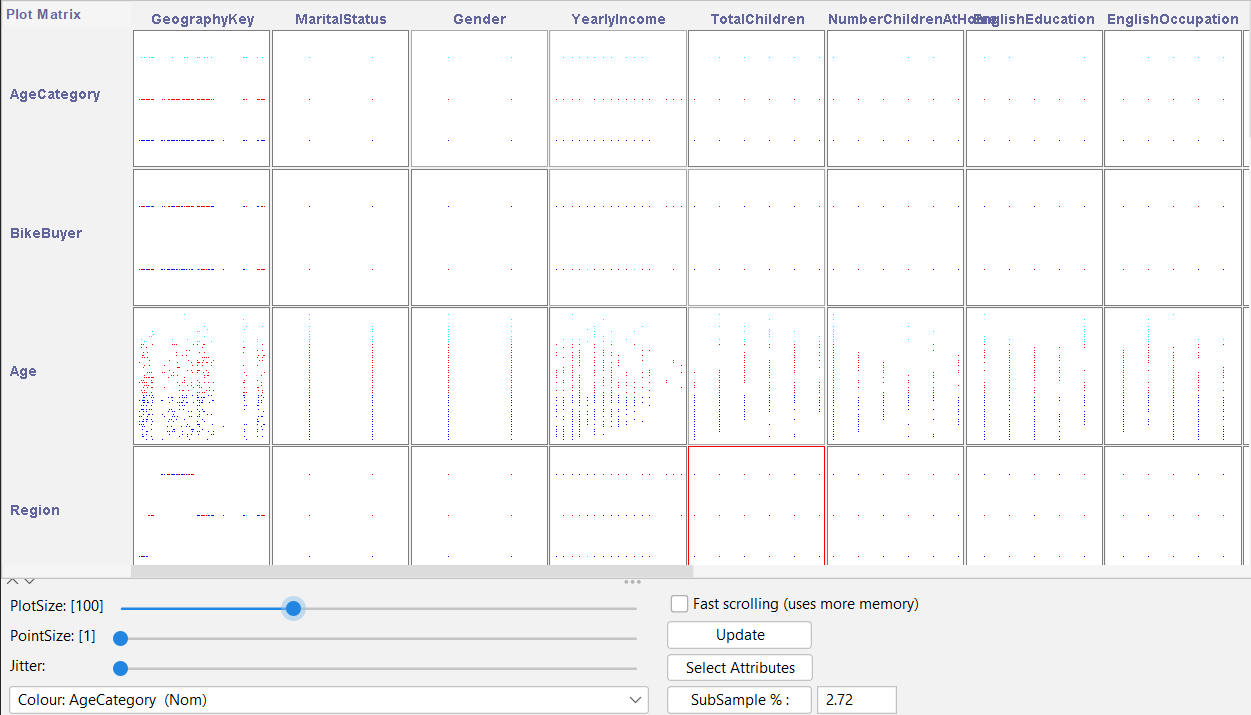
\includegraphics[width=.6\textwidth]{Visualizacion.PNG}
    \label{fig:my_label}
\end{figure}

\subsection{Ranking}

\begin{figure}[h!]
    \centering
    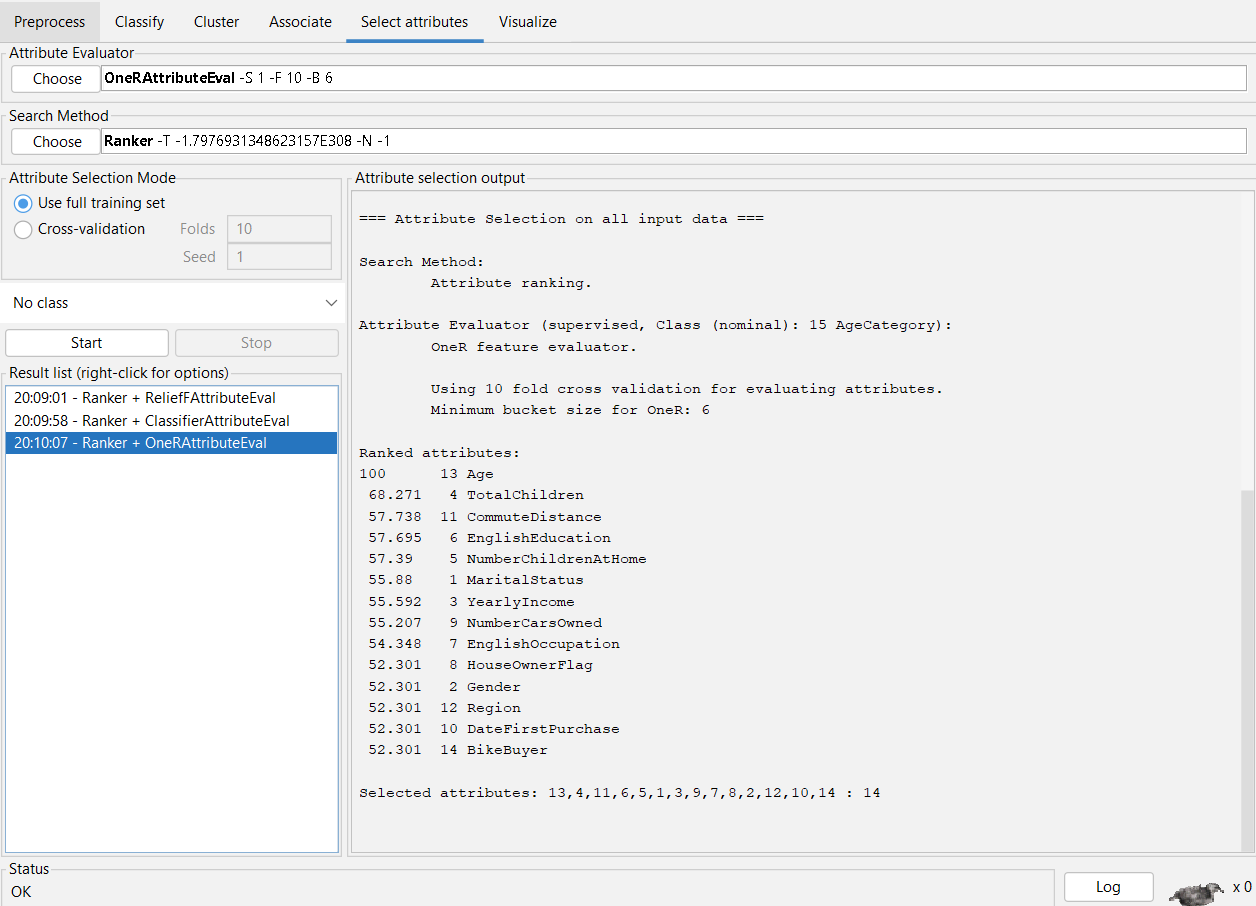
\includegraphics[width=.6\textwidth]{ranking.PNG}
    \label{fig:my_label}
\end{figure}

\clearpage

\subsection{K-means}

\begin{figure}[h!]
    \centering
    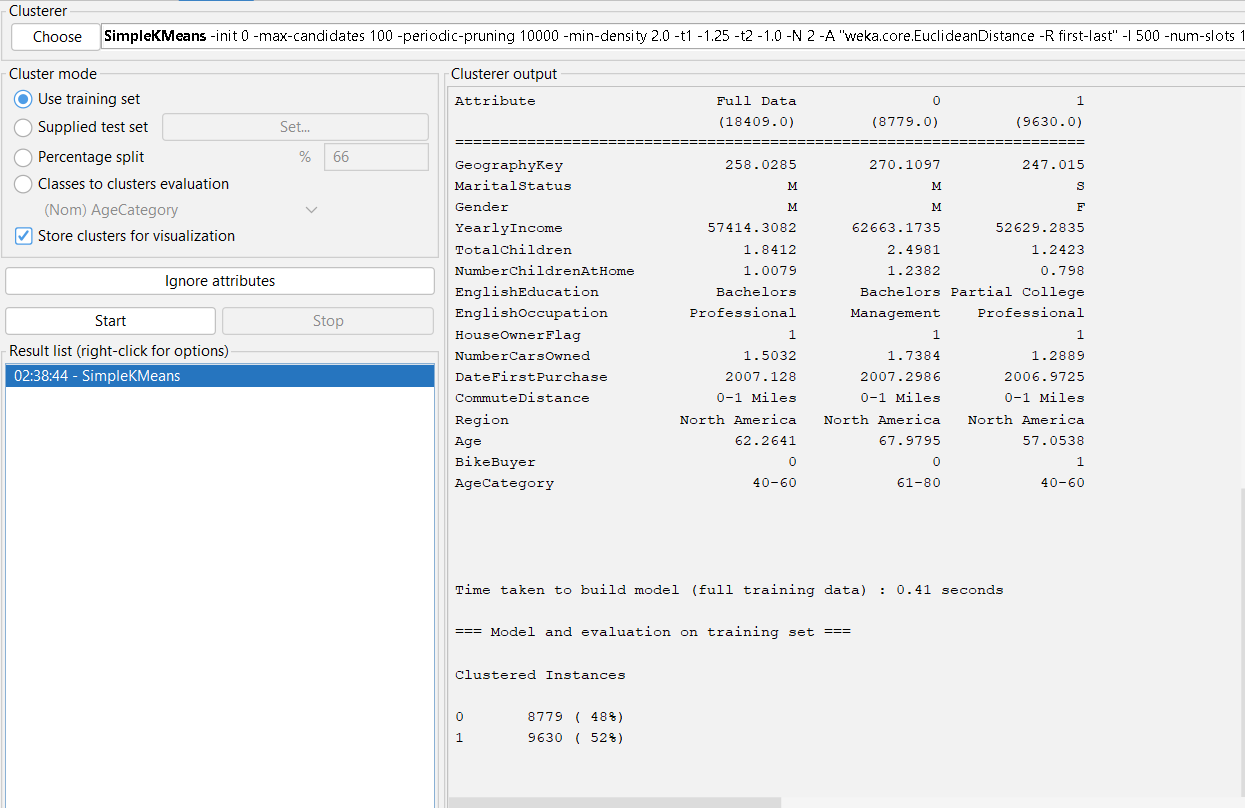
\includegraphics[width=.6\textwidth]{K-Means.PNG}
    \label{fig:my_label}
\end{figure}

En cuanto al clustering, podemos ver como se han creado dos instancias de clusters. 0 y 1, donde 0 representa aquella parte de los datos
que no han comprado una bicicleta y 1 los que sí. Podemos ver la media de cada uno de los atributos que han sido seleccionados.
Según las medias que hemos sacado, no podemos ver mucha diferencia entre los que han comprado una bicicleta y los que no. Si acaso,
podemos decir que la ocupación difiere al igual que el estado civil. También la edad difere un poco, pero no es una diferencia muy grande.
Por lo demás no hay gran cosa a destacar.

\subsection{KNN}

\begin{figure}[h!]
    \centering
    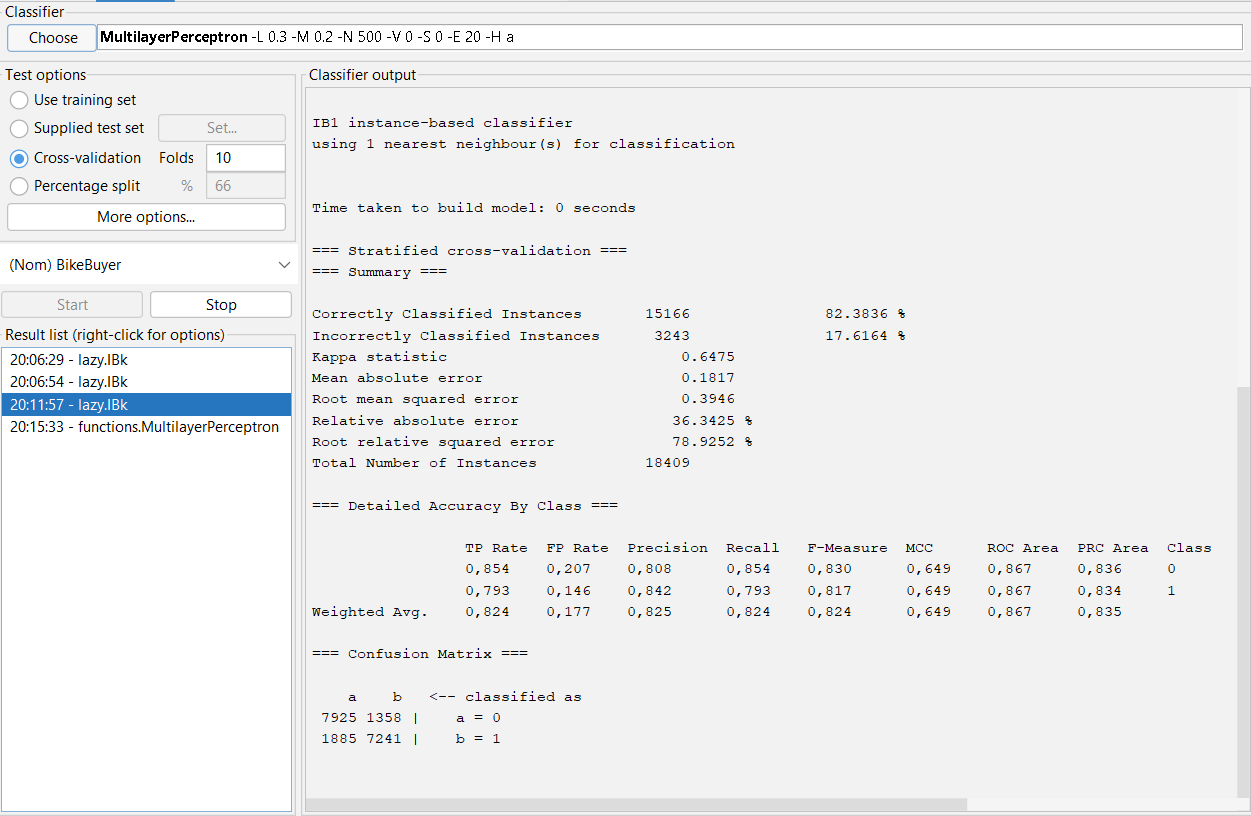
\includegraphics[width=.6\textwidth]{KNN.PNG}
    \label{fig:my_label}
\end{figure}

En el KNN podemos ver como salida la matriz de confusión. En ella podemos ver como se han clasificado los datos. En la diagonal principal
podemos ver los aciertos y en la diagonal secundaria los fallos. En este caso, con los que han comprado una bicicleta podemos observar
como ha clasificado correctamente una diferencia muy grande.

\subsection{A priori (reglas de asociación)}

\begin{figure}[h!]
    \centering
    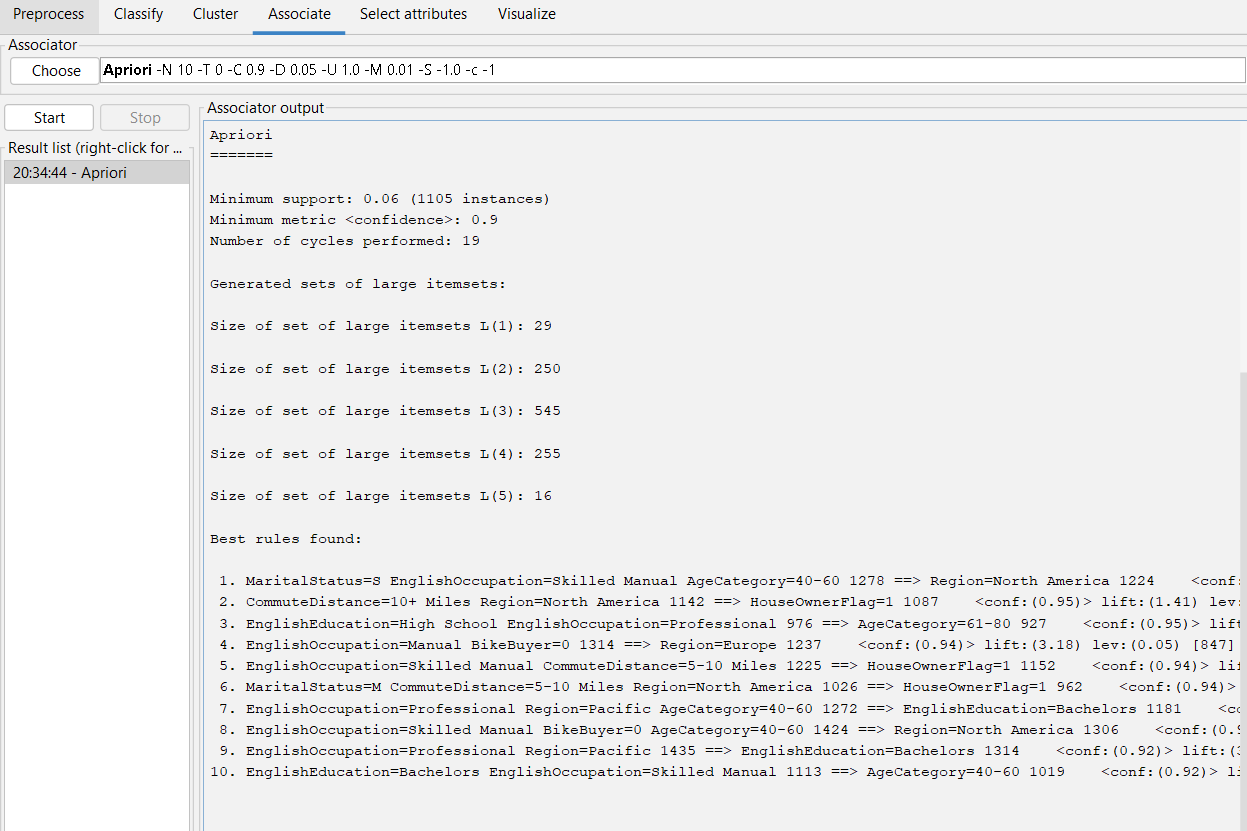
\includegraphics[width=.6\textwidth]{apriori.PNG}
    \label{fig:my_label}
\end{figure}

Con este algoritmo podemos ver las reglas de asociación que se han creado. En este caso, podemos ver las 10 reglas que se han creado.
Podemos observar como la mayoría de las reglas su principal relación es por la ocupación. Un par por la educación, otras por el estado civil
y una última por la distancia común.

\subsection{RN (Perceptrón)}

\begin{figure}[h!]
    \centering
    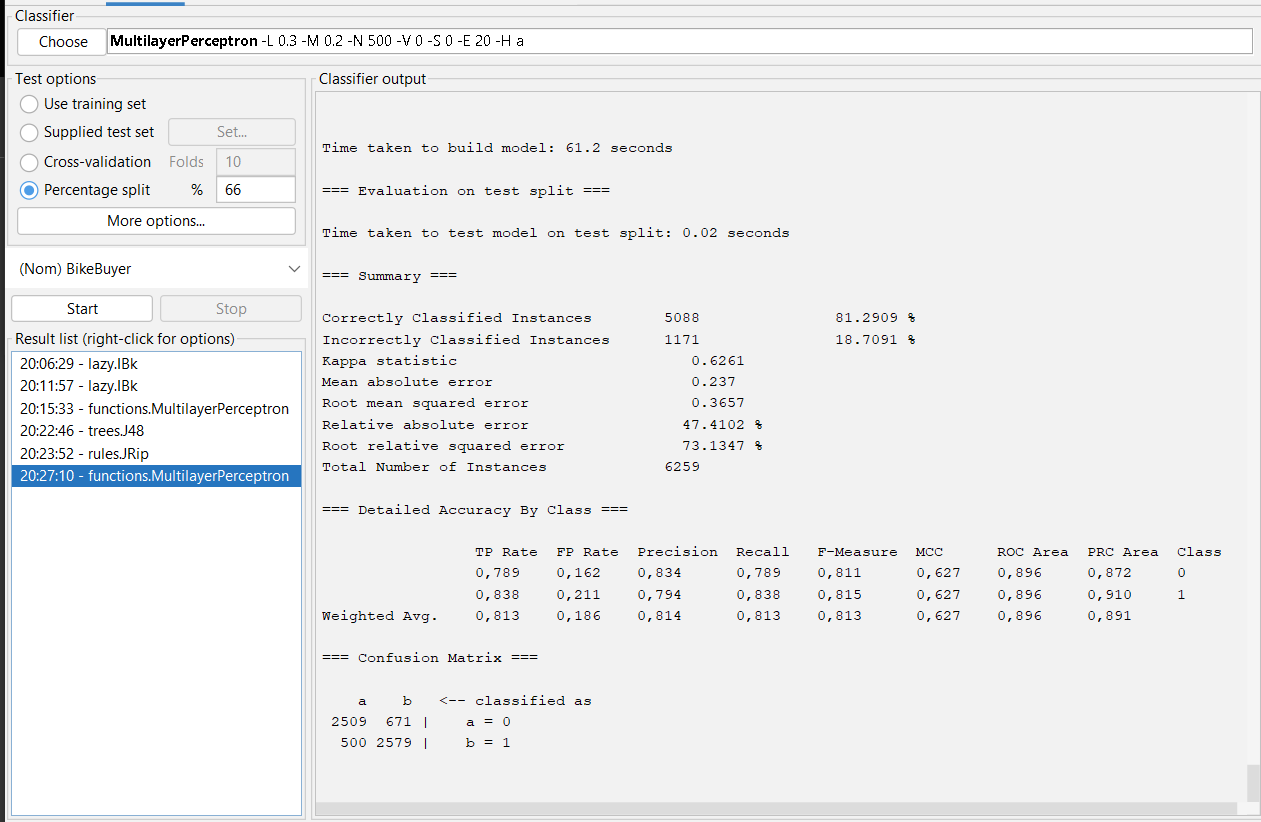
\includegraphics[width=.6\textwidth]{Multilayer.PNG}
    \label{fig:my_label}
\end{figure}

El Perceptrón nos muestra la matriz de confusión. En ella podemos ver como se han clasificado los datos. En la diagonal principal
podemos ver los aciertos y en la diagonal secundaria los fallos. En este caso, con los que han comprado una bicicleta podemos observar
como ha clasificado correctamente una diferencia muy grande.

\clearpage

\subsection{Árbol de decisión (C4.5)}

\begin{figure}[h!]
    \centering
    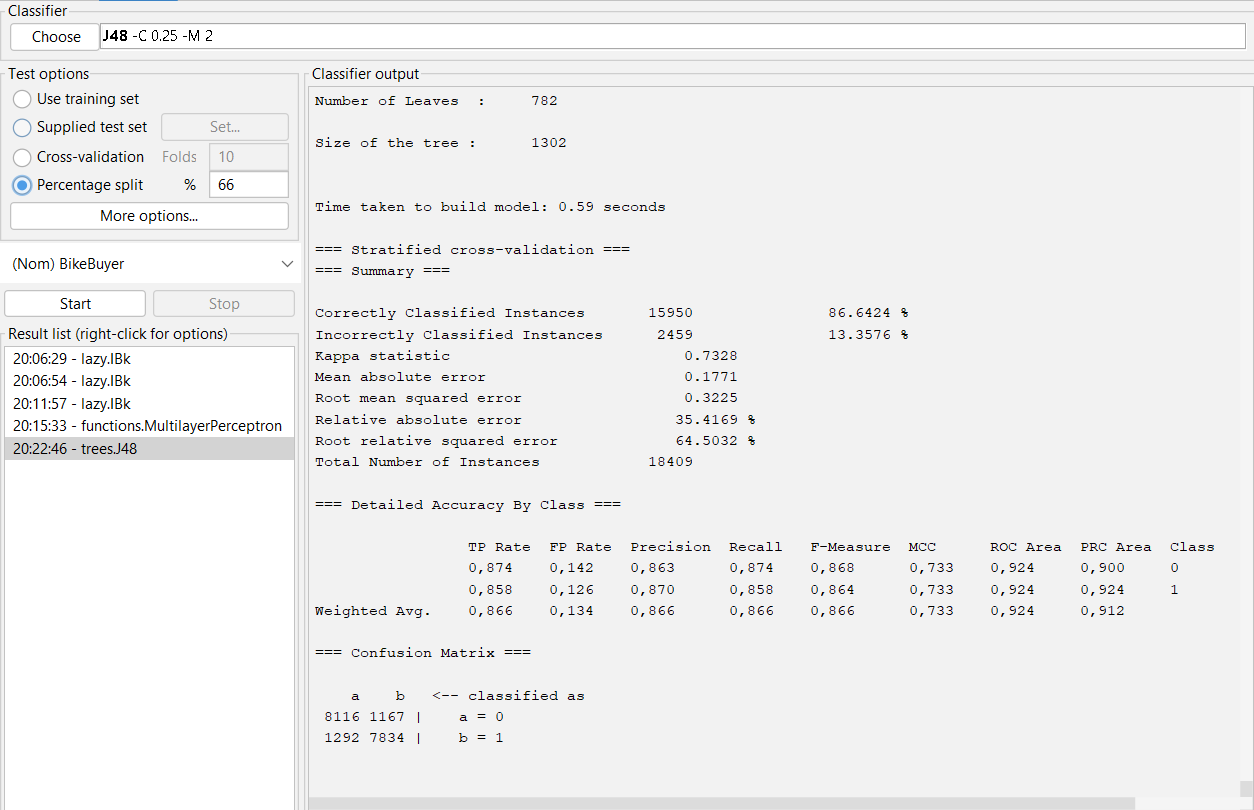
\includegraphics[width=.6\textwidth]{treeJ48.PNG}
    \label{fig:my_label}
\end{figure}

El árbol de decisión nos muestra como se ha clasificado los datos. En este caso, podemos ver como se ha clasificado a los que han comprado
una bicicleta y los que no. Podemos ver como la edad es el atributo más importante para clasificar a los que han comprado una bicicleta.
También podemos ver como la ocupación y el estado civil son importantes para clasificar a los que no han comprado una bicicleta.

\end{document}
